%\part{Grundlagen} 

%----------------------------------------------------------------------------
\section{OOP Grundlagen}
\begin{frame}[fragile]
	\frametitle{OOP Grundlagen}
	\huge OOP Grundlagen
\end{frame}

\begin{frame}
\frametitle{Einstieg in die objektorientierte Programmierung}
	\begin{block}{Objektorientierte Programmierung}
		\begin{itemize}
		  \item Modularer Programmaufbau
		  \item Die einzelnen Module hei"sen Objekte
		  \item Objekte haben Daten und Methoden
		  \item Objekte erlauben den Aufbau komplexer Programme
		\end{itemize}
	\end{block}
	\begin{exampleblock}{Erh\"ohte Abstraktion}
		\begin{itemize}
		  \item OOP erm\"oglicht die Abbildung von Problemen auf Modelle der Realit\"at 
		  \item Fokus auf die fachliche Aufgabenstellung
		\end{itemize}
	\end{exampleblock} 
\end{frame} 

\subsection{Grundbegriffe}
\begin{frame}[fragile]
	\frametitle{Grundbegriffe}
	\huge Grundbegriffe
\end{frame}
\begin{frame}
\frametitle{Objekte, Methoden und Attribute in der OOP}
	\center
	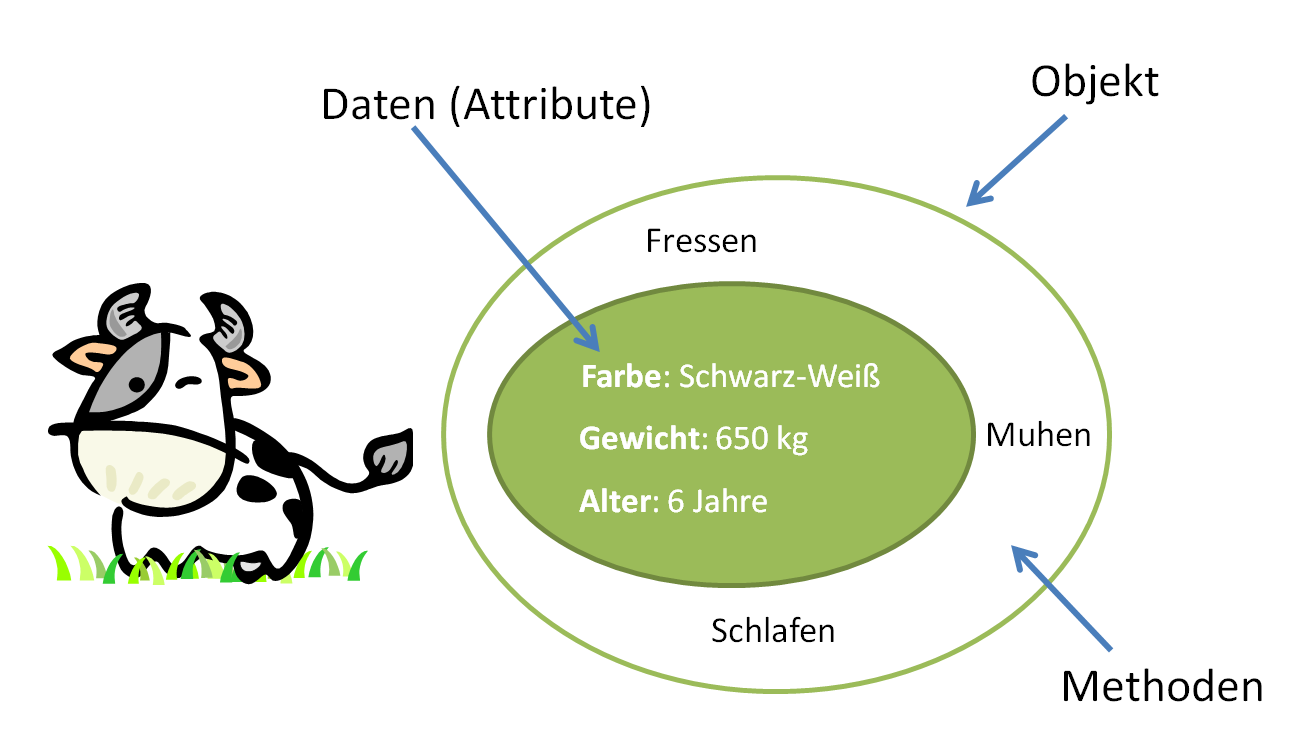
\includegraphics[width=0.9\textwidth, keepaspectratio=true]{bilder/kuh.png}
\end{frame}  
  
\begin{frame}
\frametitle{Klassen als Objektbauplan}
	\begin{columns}
	    \begin{column}{.6\textwidth}
			\small
			\begin{itemize}
			  \item Klasse fungiert als Bauplan f\"ur Objekte
			  \item Aus diesem Bauplan lassen sich beliebig viele Objekte erzeugen
			  \item Objekte aus einer Klasse besitzen die gleichen Methoden
			  \item Objekte aus einer Klasse besitzen die gleichen Attribute \\(Werte
			  k\"onnen jedoch variieren)
			  \item Klassen k\"onnen durch Vererbung weiter spezialisiert werden
			\end{itemize}
			\normalsize
	    \end{column}
	    \begin{column}{.4\textwidth}
	   		\center
			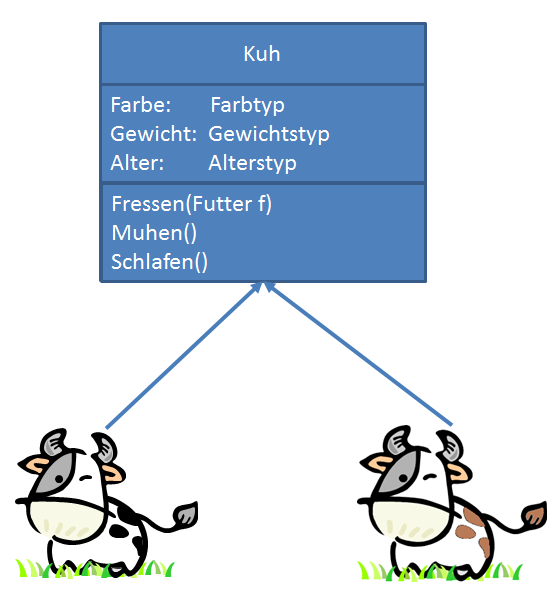
\includegraphics[width=\textwidth,
			keepaspectratio=true]{bilder/kuh_klasse.png}
	    \end{column}
	\end{columns} 
\end{frame}

\begin{frame}
\frametitle{Beziehungen zwischen Objekten}
\begin{columns}
	    \begin{column}{.6\textwidth}
			\small
			\begin{itemize}
			  \item Zwischen Objekten k\"onnen Beziehungen existieren
			  \begin{item}
			  		Beziehung zwischen Bauer und Kuh:
					\begin{enumerate}
					  \item \tiny Der Bauer kann 0 bis n K\"uhe besitzen
					  \item \tiny Eine Kuh geh\"ort genau einem Bauer
					  \item \tiny Keine Kuh kann einen Bauer besitzen \\ (gerichtete Beziehung)
					\end{enumerate}
			  \end{item} 
			\end{itemize}
			\normalsize
	    \end{column}
	    \begin{column}{.4\textwidth}
	   		\center
			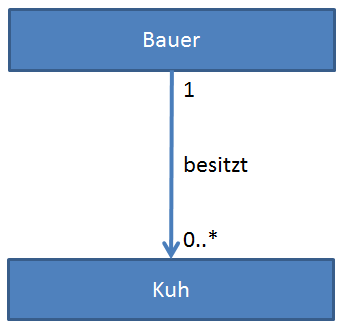
\includegraphics[width=0.9\textwidth,
			keepaspectratio=true]{bilder/asso_kuh.png}
	    \end{column}
	\end{columns} 
\end{frame}

\begin{frame}
\frametitle{Methodenaufrufe}
\begin{columns}
	    \begin{column}{.6\textwidth}
			\small
			\begin{itemize}
			  \item Objekte k\"onnen sich untereinander Botschaften senden
			  \item Damit wird der Empf\"anger aufgefordert etwas auszuf\"uhren
			  \begin{item}
			  		Erweitern wir die Klasse ''Kuh''
					\begin{enumerate}
					  \item \tiny Kuh bekommt die Methode: ''gebeMilch''
					  \item \tiny ''gebeMilch'' gibt ein Objekt vom Typ ''Milchtyp'' zur\"uck
					\end{enumerate}
			  \end{item}
			  \item Der Bauer l\"ost durch senden einer Botschaft die Methode
			  ''gebeMilch'' aus
			  \item Die Kuh f\"uhrt die Methode aus und gibt Milchtyp-Objekt zur\"uck
			\end{itemize}
			\normalsize
	    \end{column}
	    \begin{column}{.4\textwidth}
	   		\center
			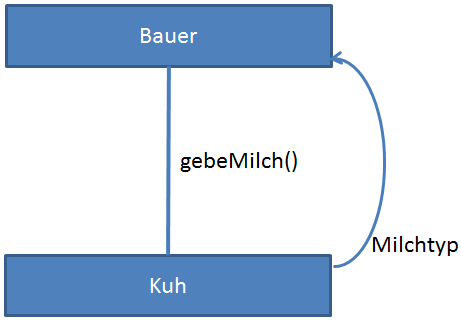
\includegraphics[width=1\textwidth,
			keepaspectratio=true]{bilder/methodenaufruf.png}
	    \end{column}
	\end{columns} 
\end{frame}
 
\subsection{Grundprinzipien}
\begin{frame}
\frametitle{Die Grundprinzipien der OOP}
\begin{itemize} 
  \item Kapselung\linebreak
  \item Vererbung\linebreak
  \item Polymorphismus\linebreak
\end{itemize}
\end{frame} 

\begin{frame}
\frametitle{Das Prinzip der Kapselung (Geheimnisprinzip)}
\begin{columns}
    \begin{column}{.5\textwidth}
		\small
		\begin{itemize}
		  \item Attribute sind von Methoden gekapselt
		  \item Damit sind die Methoden die Schnittstellen zur
		  		Au"senwelt
		  \item Dient dem kontrollierten Zugriff auf Attribute und Logik
		  \item Reduziert die Komplexit\"at da interne Strukturen verborgen bleiben
		\end{itemize}
	\end{column}
	\begin{column}{.5\textwidth} 
		\center
		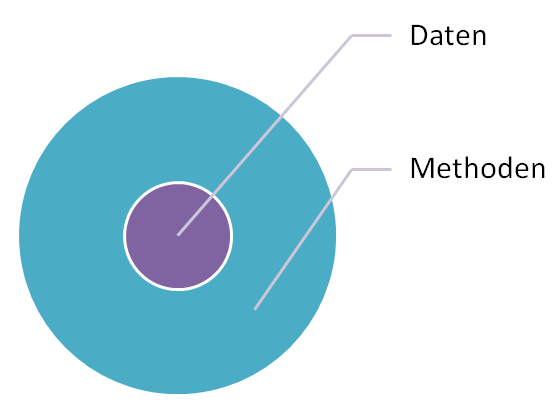
\includegraphics[width=1\textwidth,
		keepaspectratio=true]{bilder/kapselung.png}
	\end{column}
\end{columns}
\end{frame}

\begin{frame}
\frametitle{Das Prinzip der Vererbung}
\begin{columns}
	\begin{column}{.5\textwidth}
		\small
		\begin{itemize} 
		  	\item Klassen lassen sich durch Vererbung spezialisieren
		  	\item Alle Attribute und Methoden der Vaterklasse sind
			  	  Attribute und Methoden der Subklasse \\ (Die Kind-Klasse
			  	  ''erbt'')
		  	\item Funktionalit\"at der Vaterklasse bleibt vorhanden, nur die
		  		  Unterschiede werden definiert
		\end{itemize}
	\end{column}
 	\begin{column}{.5\textwidth} 
		\center
		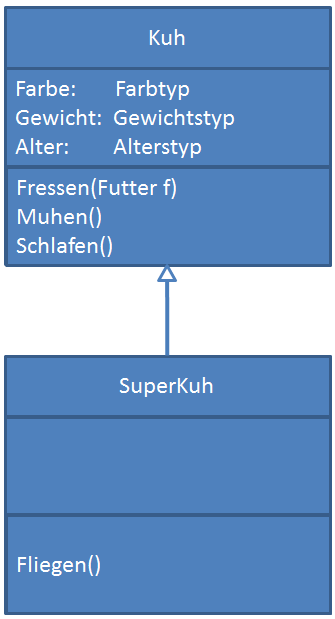
\includegraphics[width=0.5\textwidth, 
		keepaspectratio=true]{bilder/vererbung_kuh.png} 
	\end{column}
\end{columns}
\end{frame}

\begin{frame}[fragile]
\frametitle{Das Prinzip des Polymorphismus}
\begin{columns}
	\begin{column}{.4\textwidth}
		\small
		\begin{itemize} 
		  	\item Die Subklasse kann \"uberall dort genutzt werden, wo auch die
		  	Superklasse genutzt wird
		  	\item Damit wird zur Laufzeit entschieden aus welcher Klasse die Methode
		  	kommt
			\item Dieses Prinzip wird als ''sp\"ate Bindung'' bezeichnet
		\end{itemize}
	\end{column}
 	\begin{column}{.6\textwidth} 
		\begin{lstlisting}
			// Instanz einer normalen Kuh
			// Kuh-Referenz zeig auf Kuh
			Kuh kuh = new Kuh();
			
			// Instanz einer SuperKuh
			// Kuh-Referenz zeigt auf 
			// SuperKuh(Polymorphie)
			Kuh sKuh = new SuperKuh();
			
			// Eine normale Kuh schlaeft 
			// 4 Stunden am Tag
			kuh.schlafen();
			
			// Superkuehe schlafen nur 
			// 1 Stunde am Tag
			sKuh.schlafen();
		\end{lstlisting}
	\end{column}
\end{columns}
\end{frame}

\begin{frame}
	\frametitle{Zeit f\"ur eine \"Ubung}
	\center
	
\includegraphics[width=0.8\textwidth,
	keepaspectratio=true]{bilder/uebung.png}
\end{frame}